\documentclass[11pt]{scrartcl}
\usepackage[T1]{fontenc}
\usepackage[a4paper, left=3cm, right=2cm, top=2cm, bottom=2cm]{geometry}
\usepackage[activate]{pdfcprot}
\usepackage[ngerman]{babel}
\usepackage[parfill]{parskip}
\usepackage[utf8]{inputenc}
\usepackage{kurier}
\usepackage{amsmath}
\usepackage{amssymb}
\usepackage{xcolor}
\usepackage{epstopdf}
\usepackage{txfonts}
\usepackage{fancyhdr}
\usepackage{graphicx}
\usepackage{prettyref}
\usepackage{hyperref}
\usepackage{eurosym}
\usepackage{setspace}
\usepackage{units}
\usepackage{eso-pic,graphicx}
\usepackage{icomma}

\definecolor{darkblue}{rgb}{0,0,.5}
\hypersetup{pdftex=true, colorlinks=true, breaklinks=false, linkcolor=black, menucolor=black, pagecolor=black, urlcolor=darkblue}



\setlength{\columnsep}{2cm}


\newcommand{\arcsinh}{\mathrm{arcsinh}}
\newcommand{\asinh}{\mathrm{arcsinh}}
\newcommand{\ergebnis}{\textcolor{red}{\mathrm{Ergebnis}}}
\newcommand{\fehlt}{\textcolor{red}{Hier fehlen noch Inhalte.}}
\newcommand{\betanotice}{\textcolor{red}{Diese Aufgaben sind noch nicht in der Übung kontrolliert worden. Es sind lediglich meine Überlegungen und Lösungsansätze zu den Aufgaben. Es können Fehler enthalten sein!!! Das Dokument wird fortwährend aktualisiert und erst wenn das \textcolor{black}{beta} aus dem Dateinamen verschwindet ist es endgültig.}}
\newcommand{\half}{\frac{1}{2}}
\renewcommand{\d}{\, \mathrm d}
\newcommand{\punkte}{\textcolor{white}{xxxxx}}
\newcommand{\p}{\, \partial}
\newcommand{\dd}[1]{\item[#1] \hfill \\}

\renewcommand{\familydefault}{\sfdefault}
\renewcommand\thesection{}
\renewcommand\thesubsection{}
\renewcommand\thesubsubsection{}


\newcommand{\themodul}{CAM - Fragen-Antworten}
\newcommand{\thetutor}{Martina Klocke}

\pagestyle{fancy}
\fancyhead[L]{\footnotesize{C. Hansen}}
\chead{\thepage}
\rhead{}
\lfoot{}
\cfoot{}
\rfoot{}

\title{\themodul{}, \thetutor}


\author{Christoph Hansen \\ {\small \href{mailto:uni@christophhansen.eu}{uni@christophhansen.eu}} }

\date{}


\begin{document}

\maketitle

Dieser Text ist unter dieser \href{http://creativecommons.org/licenses/by-nc-sa/3.0/}{Creative Commons} Lizenz veröffentlicht.


\tableofcontents

\newpage

\section{Einführung CAM}

\subsection*{Beschreiben des Produktlebenszyklus: 
Phasen. Wie verhalten sich Umsatz und Gewinn in Abhängigkeit von der 
jeweiligen Phase. Begründen Sie Ihre Aussage. }


\begin{figure}[h]
\centering
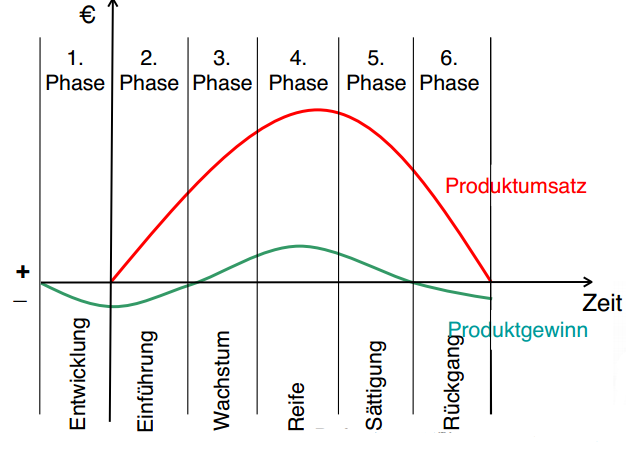
\includegraphics[scale=0.7]{Bild1_1.png}
\end{figure}


In der Graphik können wir die einzelnen Phasen ablesen, in der Entwicklung kostet das Produkt Geld, da wir Leute, Maschinen etc für die Entwicklung bezahlen müssen. Auch in der Einführungsphase beginnt der Umsatz zu steigen, allerdings kostet uns das Produkt noch Geld, da wir Geld in Werbung und oftmals Ausbesserungen stecken müssen. In der Wachstumsphase fangen wir an mit dem Produkt Geld zu verdienen, was in der Phase der Produktreife zu einem Umsatz als auch Gewinnmaximum führt. In den Phasen der Sättigung und des Rückgangs sinken der Umsatz als auch der Gewinn wieder. Zum Schluss kostet uns das Produkt wieder Geld, da wir trotz wenig bis keinen Verkäufen noch Support oder Garantieleistungen erfüllen müssen.


\subsection*{Welche Potenziale kann der Anwender von der Kopplung CAD/CAM erwarten? 
(fünf Beispiele) }


\begin{itemize}
\item[1)] die direkte Anbindung an die Fertigung ermöglicht einen direkteren Austausch zwischen den Konstrukteuren und den Leuten an der Maschine
\item[2)] Kostensenkung: durch weniger Fehlkonstruktionen
\item[3)] Zeitersparnis: es kann schon mit CAM angefangen werden bevor CAD komplett fertig ist
\item[4)] keine Datenumwandlungen: bei verschiedenen Systemen bei CAD und CAM kann es sein, das man Daten umwandeln muss, dabei gehen oft Parameter und/oder Daten verloren
\item[5)] schnelle Ermittlung von Problemen
\end{itemize}

\newpage

\subsection*{Was bedeuten die Kürzel und welche Tätigkeiten werden mit diesen Systemen 
unterstützt?  
Produkt entwerfen -> CAD -> CAE -> CAP -> CAM -> Produkt }


\begin{itemize}
\item[\textbf{CAD:}] Computer Aided Design $\Rightarrow$ Konstruieren am Rechner
\item[\textbf{CAE:}] Computer Aided Engineering $\Rightarrow$ umfasst alle Varianten der Rechner-Unterstützung von Arbeitsprozessen in der Technik.
\item[\textbf{CAP:}] Computer Aided Process Planning $\Rightarrow$ Werkzeugmaschinen belegen, Fertigungsmittel bereitstellen
\item[\textbf{CAM:}] Computer Aided Manufacturing $\Rightarrow$ Spannvorrichtung festlege, Werkzeuge auswählen, Arbeitspläne erstellen, NC-Progs simulieren und bereitstellen, Produkt herstellen
\end{itemize}


\subsection*{Welche Informationen / Unterlagen erhalten Sie aus den Bereichen CAD, CAE, 
CAP, CAM? }

\begin{itemize}
\item[\textbf{CAD:}] Zeichnungen, Stücklisten
\item[\textbf{CAE:}] Montagepläne, Doku
\item[\textbf{CAP:}] Maschinenbelegung, Arbeitspläne
\item[\textbf{CAM:}] NC-Programme, Werkzeuglisten, Bestückungspläne, Korrekturen
\end{itemize}


\newpage

\section{NC-Programmierung}


\subsection*{Was bedeuten die Kürzel: CNC, DNC, LAN?}

\begin{itemize}
\item[\textbf{CNC:}] Computerized Numerical Control
\item[\textbf{DNC:}] Direct Numerical Control
\item[\textbf{LAN:}] Local Area Network
\end{itemize}




\end{document}